%%
%% This is file `sample-sigconf.tex',
%% generated with the docstrip utility.
%%
%% The original source files were:
%%
%% samples.dtx  (with options: `sigconf')
%% 
%% IMPORTANT NOTICE:
%% 
%% For the copyright see the source file.
%% 
%% Any modified versions of this file must be renamed
%% with new filenames distinct from sample-sigconf.tex.
%% 
%% For distribution of the original source see the terms
%% for copying and modification in the file samples.dtx.
%% 
%% This generated file may be distributed as long as the
%% original source files, as listed above, are part of the
%% same distribution. (The sources need not necessarily be
%% in the same archive or directory.)
%%
%% The first command in your LaTeX source must be the \documentclass command.
\documentclass[sigconf]{acmart}

%%
%% \BibTeX command to typeset BibTeX logo in the docs
\AtBeginDocument{%
  \providecommand\BibTeX{{%
    \normalfont B\kern-0.5em{\scshape i\kern-0.25em b}\kern-0.8em\TeX}}}

%% Rights management information.  This information is sent to you
%% when you complete the rights form.  These commands have SAMPLE
%% values in them; it is your responsibility as an author to replace
%% the commands and values with those provided to you when you
%% complete the rights form.
\setcopyright{acmcopyright}
\copyrightyear{2018}
\acmYear{2018}
\acmDOI{10.1145/1122445.1122456}

%% These commands are for a PROCEEDINGS abstract or paper.
\acmConference[Woodstock '18]{Woodstock '18: ACM International Conference of Human-Robot Interaction}{8 March 2021}{Online}
\acmBooktitle{Woodstock '18: ACM International Conference of Human-Robot Interaction,
8 March 2021, Online}
\acmPrice{15.00}
\acmISBN{978-1-4503-XXXX-X/18/06}

\graphicspath{{../figures}} %goes to path: figures/

%%
%% Submission ID.
%% Use this when submitting an article to a sponsored event. You'll
%% receive a unique submission ID from the organizers
%% of the event, and this ID should be used as the parameter to this command.
%%\acmSubmissionID{123-A56-BU3}

%%
%% The majority of ACM publications use numbered citations and
%% references.  The command \citestyle{authoryear} switches to the
%% "author year" style.
%%
%% If you are preparing content for an event
%% sponsored by ACM SIGGRAPH, you must use the "author year" style of
%% citations and references.
%% Uncommenting
%% the next command will enable that style.
%%\citestyle{acmauthoryear}

%%
%% end of the preamble, start of the body of the document source.
\begin{document}

%%
%% The "title" command has an optional parameter,
%% allowing the author to define a "short title" to be used in page headers.
\title{air4children: Artificial Intelligence and Robotics for Children}

%%
%% The "author" command and its associated commands are used to define
%% the authors and their affiliations.
%% Of note is the shared affiliation of the first two authors, and the
%% "authornote" and "authornotemark" commands
%% used to denote shared contribution to the research.

%\author{Ben Trovato}
%\authornote{Both authors contributed equally to this research.}
%\email{trovato@corporation.com}
%\orcid{1234-5678-9012}
%\author{G.K.M. Tobin}

\author{Co-author A}
\affiliation{%
  \institution{University of A}
  \streetaddress{Adress}
  \city{City}
  \country{Country}}
\email{email@internet.org}

\author{Co-author B}
\affiliation{%
\institution{University of A}
\streetaddress{Adress}
\city{City}
\country{Country}}
\email{email@internet.org}

\author{Miguel Xochicale}
\affiliation{%
  \institution{King's College London}
  \city{London}
  \country{UK}}
\authornotemark[1]
\email{miguel.xochicale@kcl.ac.uk}

%%
%% By default, the full list of authors will be used in the page
%% headers. Often, this list is too long, and will overlap
%% other information printed in the page headers. This command allows
%% the author to define a more concise list
%% of authors' names for this purpose.
\renewcommand{\shortauthors}{Xochicale M. et al.}

%%
%% The abstract is a short summary of the work to be presented in the
%% article.
\begin{abstract}
  A clear and well-documented \LaTeX\ document is presented as an
  article formatted for publication by ACM in a conference proceedings
  or journal publication. Based on the ``acmart'' document class, this
  article presents and explains many of the common variations, as well
  as many of the formatting elements an author may use in the
  preparation of the documentation of their work.
  A clear and well-documented \LaTeX\ document is presented as an
  article formatted for publication by ACM in a conference proceedings
  or journal publication. Based on the ``acmart'' document class, this
  article presents and explains many of the common variations, as well
  as many of the formatting elements an author may use in the
  preparation of the documentation of their work.
\end{abstract}

%%
%% The code below is generated by the tool at http://dl.acm.org/ccs.cfm.
%% Please copy and paste the code instead of the example below.
%%
\begin{CCSXML}
<ccs2012>
     <concept>
         <concept_id>10003120.10003121.10011748</concept_id>
         <concept_desc>Human-centered computing~Empirical studies in HCI</concept_desc>
         <concept_significance>500</concept_significance>
         </concept>
     <concept>
         <concept_id>10003120.10011738.10011776</concept_id>
         <concept_desc>Human-centered computing~Accessibility systems and tools</concept_desc>
         <concept_significance>500</concept_significance>
         </concept>
     <concept>
         <concept_id>10010405.10010489.10010491</concept_id>
         <concept_desc>Applied computing~Interactive learning environments</concept_desc>
         <concept_significance>300</concept_significance>
         </concept>
     <concept>
         <concept_id>10003456.10010927.10010930.10010931</concept_id>
         <concept_desc>Social and professional topics~Children</concept_desc>
         <concept_significance>500</concept_significance>
         </concept>
     <concept>
         <concept_id>10010147.10010178.10010187.10010194</concept_id>
         <concept_desc>Computing methodologies~Cognitive robotics</concept_desc>
         <concept_significance>300</concept_significance>
         </concept>
</ccs2012>
\end{CCSXML}

\ccsdesc[500]{Human-centered computing~Empirical studies in HCI}
\ccsdesc[500]{Human-centered computing~Accessibility systems and tools}
\ccsdesc[300]{Applied computing~Interactive learning environments}
\ccsdesc[500]{Social and professional topics~Children}
\ccsdesc[300]{Computing methodologies~Cognitive robotics}

%%
%% Keywords. The author(s) should pick words that accurately describe
%% the work being presented. Separate the keywords with commas.
\keywords{Child-robot interaction, child-centred AI, Educational Robotics}

%% A "teaser" image appears between the author and affiliation
%% information and the body of the document, and typically spans the
%% page.
\begin{teaserfigure}
  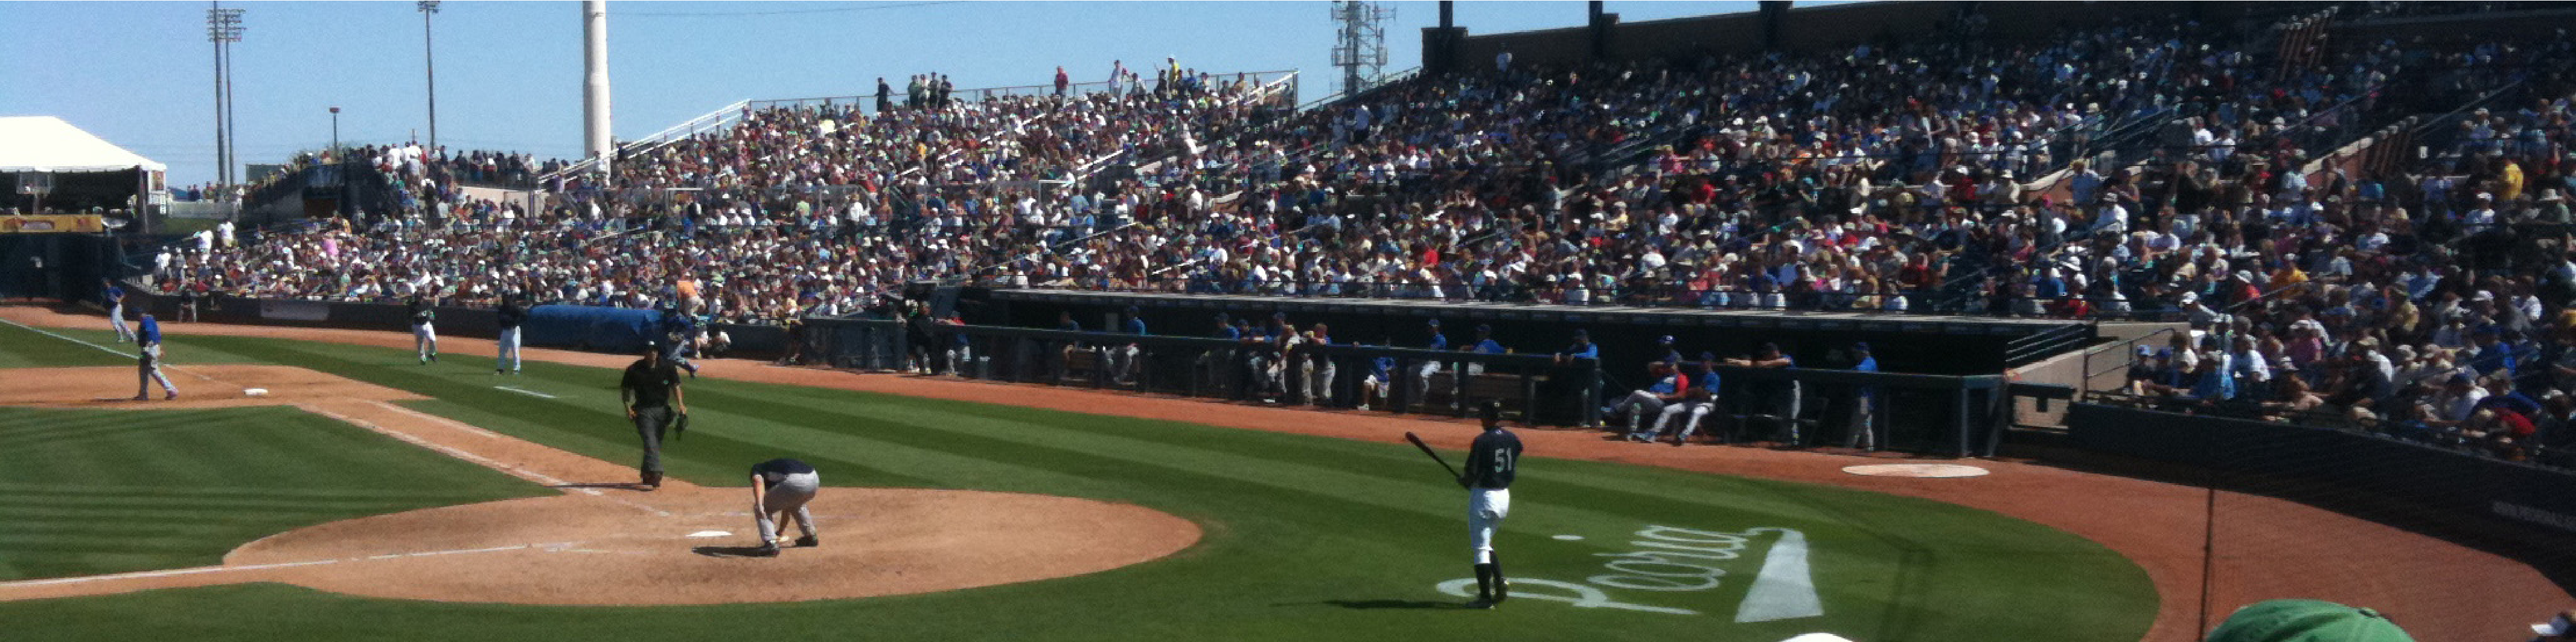
\includegraphics[width=\textwidth]{sampleteaser}
  \caption{Seattle Mariners at Spring Training, 2010.}
  \Description{Enjoying the baseball game from the third-base
  seats. Ichiro Suzuki preparing to bat.}
  \label{fig:teaser}
\end{teaserfigure}

%%
%% This command processes the author and affiliation and title
%% information and builds the first part of the formatted document.
\maketitle

\section{Introduction}

Current progress in the fields of Artificial Intelligence and Robotics (AIR)
is accelerating specially in countries where innonavtion and technologies are happenigs. 
However, even thought these fields are growing work is in progress in separated streams
for AI and Robotics, there is little work that put together both fields and with
little to none focus on children. With this in mind this work is proposing 
the term AIR4children in a way to offer pedagogical, open-source software and hardware
tools to balance the current posiblities for children to enjoy and to dicover these 
fields from a children-like perspective.
As pointed in the guidance of AI for children by UNICEF \cite{UNICEF2020},
there are many challenges to make inclusive AIR, in this case, 
from any or idealialy under-represented communities and provie fairness and non-discrimination 
in child-robot interaction as well as design curriculums for children of different 
socieconomical backgrounds, developmental stages or learning abilitities. 
The aim of the AIR4children is to prepare children for present 
to contribute to resposnbile AIR for the present and the future.

Anoother aspects as the socialbitly of robots are well explamplied with 
Jibo [REF], Cosmos [REF] and more recently Shelly, a tortoise-like robot, to tacke 
multiple interaction of one-to-many as well the resctrition of children
abusive behaviours towards robots \cite{hu2018}. 


ACM's consolidated article template, introduced in 2017, provides a

consistent \LaTeX\ style for use across ACM publications, and
incorporates accessibility and metadata-extraction functionality
necessary for future Digital Library endeavors. Numerous ACM and
SIG-specific \LaTeX\ templates have been examined, and their unique
features incorporated into this single new template.

If you are new to publishing with ACM, this document is a valuable
guide to the process of preparing your work for publication. If you
have published with ACM before, this document provides insight and
instruction into more recent changes to the article template.

The ``\verb|acmart|'' document class can be used to prepare articles
for any ACM publication --- conference or journal, and for any stage
of publication, from review to final ``camera-ready'' copy, to the
author's own version, with {\itshape very} few changes to the source.

\section{Open Source AI and Robotics}
As noted in the introduction, the ``\verb|acmart|'' document class can
be used to prepare many different kinds of documentation --- a
double-blind initial submission of a full-length technical paper, a
two-page SIGGRAPH Emerging Technologies abstract, a ``camera-ready''
journal article, a SIGCHI Extended Abstract, and more --- all by
selecting the appropriate {\itshape template style} and {\itshape
  template parameters}.

This document will explain the major features of the document
class. For further information, the {\itshape \LaTeX\ User's Guide} is
available from
\url{https://www.acm.org/publications/proceedings-template}.


\subsection{Open Source AI}
As noted in the introduction, the ``\verb|acmart|'' document class can
be used to prepare many different kinds of documentation --- a
double-blind initial submission of a full-length technical paper, a
two-page SIGGRAPH Emerging Technologies abstract, a ``camera-ready''
journal article, a SIGCHI Extended Abstract, and more --- all by
selecting the appropriate {\itshape template style} and {\itshape
  template parameters}.

\subsection{Open Source Robotics}
As noted in the introduction, the ``\verb|acmart|'' document class can
be used to prepare many different kinds of documentation --- a
double-blind initial submission of a full-length technical paper, a
two-page SIGGRAPH Emerging Technologies abstract, a ``camera-ready''
journal article, a SIGCHI Extended Abstract, and more --- all by
selecting the appropriate {\itshape template style} and {\itshape
  template parameters}.



\section{Open AIR4Children}
The ``\verb|acmart|'' document class includes the ``\verb|booktabs|''
package --- \url{https://ctan.org/pkg/booktabs} --- for preparing
high-quality tables.

Table captions are placed {\itshape above} the table.

Because tables cannot be split across pages, the best placement for
them is typically the top of the page nearest their initial cite.  To
ensure this proper ``floating'' placement of tables, use the
environment \textbf{table} to enclose the table's contents and the
table caption.  The contents of the table itself must go in the
\textbf{tabular} environment, to be aligned properly in rows and
columns, with the desired horizontal and vertical rules.  Again,
detailed instructions on \textbf{tabular} material are found in the
\textit{\LaTeX\ User's Guide}.

Immediately following this sentence is the point at which
Table~\ref{tab:freq} is included in the input file; compare the
placement of the table here with the table in the printed output of
this document.

\begin{table}
  \caption{Frequency of Special Characters}
  \label{tab:freq}
  \begin{tabular}{ccl}
    \toprule
    Non-English or Math&Frequency&Comments\\
    \midrule
    \O & 1 in 1,000& For Swedish names\\
    $\pi$ & 1 in 5& Common in math\\
    \$ & 4 in 5 & Used in business\\
    $\Psi^2_1$ & 1 in 40,000& Unexplained usage\\
  \bottomrule
\end{tabular}
\end{table}

To set a wider table, which takes up the whole width of the page's
live area, use the environment \textbf{table*} to enclose the table's
contents and the table caption.  As with a single-column table, this
wide table will ``float'' to a location deemed more
desirable. Immediately following this sentence is the point at which
Table~\ref{tab:commands} is included in the input file; again, it is
instructive to compare the placement of the table here with the table
in the printed output of this document.

\begin{table*}
  \caption{Some Typical Commands}
  \label{tab:commands}
  \begin{tabular}{ccl}
    \toprule
    Command &A Number & Comments\\
    \midrule
    \texttt{{\char'134}author} & 100& Author \\
    \texttt{{\char'134}table}& 300 & For tables\\
    \texttt{{\char'134}table*}& 400& For wider tables\\
    \bottomrule
  \end{tabular}
\end{table*}

Always use midrule to separate table header rows from data rows, and
use it only for this purpose. This enables assistive technologies to
recognise table headers and support their users in navigating tables
more easily.


\subsection{Open hardware and software}
The ``\verb|figure|'' environment should be used for figures. One or
more images can be placed within a figure. If your figure contains
third-party material, you must clearly identify it as such, as shown
in the example below.
\begin{figure}[h]
  \centering
  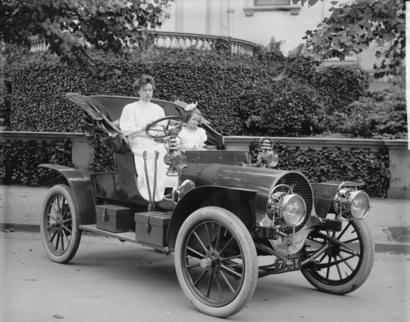
\includegraphics[width=\linewidth]{sample-franklin}
  \caption{1907 Franklin Model D roadster. Photograph by Harris \&
    Ewing, Inc. [Public domain], via Wikimedia
    Commons. (\url{https://goo.gl/VLCRBB}).}
  \Description{A woman and a girl in white dresses sit in an open car.}
\end{figure}

Your figures should contain a caption which describes the figure to
the reader.

Figure captions are placed {\itshape below} the figure.

Every figure should also have a figure description unless it is purely
decorative. These descriptions convey what’s in the image to someone
who cannot see it. They are also used by search engine crawlers for
indexing images, and when images cannot be loaded.

A figure description must be unformatted plain text less than 2000
characters long (including spaces).  {\bfseries Figure descriptions
  should not repeat the figure caption – their purpose is to capture
  important information that is not already provided in the caption or
  the main text of the paper.} For figures that convey important and
complex new information, a short text description may not be
adequate. More complex alternative descriptions can be placed in an
appendix and referenced in a short figure description. For example,
provide a data table capturing the information in a bar chart, or a
structured list representing a graph.  For additional information
regarding how best to write figure descriptions and why doing this is
so important, please see
\url{https://www.acm.org/publications/taps/describing-figures/}.

\subsection{Open teaching materials}

A ``teaser figure'' is an image, or set of images in one figure, that
are placed after all author and affiliation information, and before
the body of the article, spanning the page. If you wish to have such a
figure in your article, place the command immediately before the
\verb|\maketitle| command:
\begin{verbatim}
  \begin{teaserfigure}
    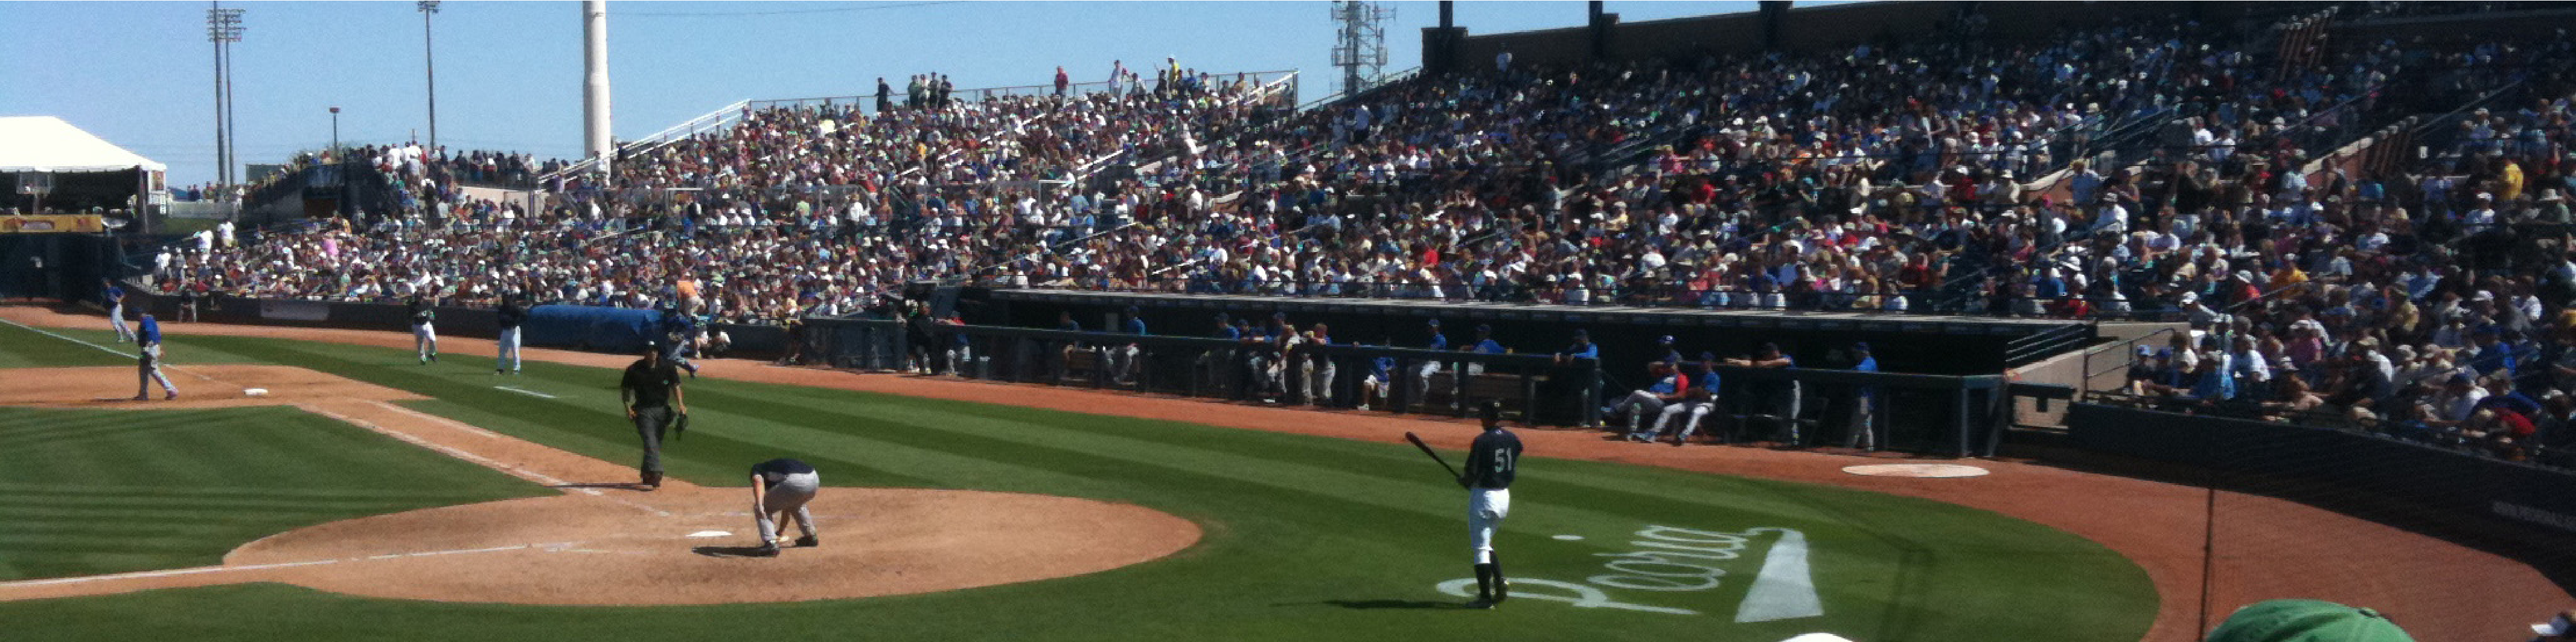
\includegraphics[width=\textwidth]{sampleteaser}
    \caption{figure caption}
    \Description{figure description}
  \end{teaserfigure}
\end{verbatim}

\section{Conclusions and future work}

The use of \BibTeX\ for the preparation and formatting of one's
references is strongly recommended. Authors' names should be complete
--- use full first names (``Donald E. Knuth'') not initials
(``D. E. Knuth'') --- and the salient identifying features of a
reference should be included: title, year, volume, number, pages,
article DOI, etc.

The bibliography is included in your source document with these two
commands, placed just before the \verb|\end{document}| command:
\begin{verbatim}
  \bibliographystyle{ACM-Reference-Format}
  \bibliography{bibfile}
\end{verbatim}
where ``\verb|bibfile|'' is the name, without the ``\verb|.bib|''
suffix, of the \BibTeX\ file.

Citations and references are numbered by default. A small number of
ACM publications have citations and references formatted in the
``author year'' style; for these exceptions, please include this
command in the {\bfseries preamble} (before the command
``\verb|\begin{document}|'') of your \LaTeX\ source:
\begin{verbatim}
  \citestyle{acmauthoryear}
\end{verbatim}

  Some examples.  A paginated journal article \cite{UNICEF2020}
  %, an
  %enumerated journal article \cite{Cohen07}, a reference to an entire
  %issue \cite{JCohen96}, a monograph (whole book) \cite{Kosiur01}, a
  %monograph/whole book in a series (see 2a in spec. document).
  %tech report: \cite{Harel78},
  %online: \cite{Thornburg01},
  %online: \cite{Ablamowicz07},
  %misc: \cite{Poker06}
  %misc: \cite{Obama08}
  %manuals:  \cite{Fear05},
  % \cite{Amsthm15}

%  \cite{Harel79}, a divisible-book such as an anthology or compilation
%  \cite{Editor00} followed by the same example, however we only output
%  the series if the volume number is given \cite{Editor00a} (so
%  Editor00a's series should NOT be present since it has no vol. no.),
%  a chapter in a divisible book \cite{Spector90}, a chapter in a
%  divisible book in a series \cite{Douglass98}, a multi-volume work as
%  book \cite{Knuth97}, a couple of articles in a proceedings (of a
%  conference, symposium, workshop for example) (paginated proceedings
%  article) \cite{Andler79, Hagerup1993}, a proceedings article with
%  all possible elements \cite{Smith10}, an example of an enumerated
%  proceedings article \cite{VanGundy07}, an informally published work
%  \cite{Harel78}, a couple of preprints \cite{Bornmann2019,
%    AnzarootPBM14}, a doctoral dissertation \cite{Clarkson85}, a
%  master's thesis: \cite{anisi03}, an online document / world wide web
% resource \cite{Thornburg01, Ablamowicz07, Poker06}, a video game
%  (Case 1) \cite{Obama08} and (Case 2) \cite{Novak03} and \cite{Lee05}
%  and (Case 3) a patent \cite{JoeScientist001}, work accepted for
%  publication \cite{rous08}, 'YYYYb'-test for prolific author
%  \cite{SaeediMEJ10} and \cite{SaeediJETC10}. Other cites might
%  contain 'duplicate' DOI and URLs (some SIAM articles)
%  \cite{Kirschmer:2010:AEI:1958016.1958018}. Boris / Barbara Beeton:
%  multi-volume works as books \cite{MR781536} and \cite{MR781537}. A
%  couple of citations with DOIs:
%  \cite{2004:ITE:1009386.1010128,Kirschmer:2010:AEI:1958016.1958018}. Online
%  citations: \cite{TUGInstmem, Thornburg01, CTANacmart}. Artifacts:
%  \cite{R} and \cite{UMassCitations}.

%%
%% The acknowledgments section is defined using the "acks" environment
%% (and NOT an unnumbered section). This ensures the proper
%% identification of the section in the article metadata, and the
%% consistent spelling of the heading.
\begin{acks}
To Robert, for the bagels and explaining CMYK and color spaces.
\end{acks}

%%
%% The next two lines define the bibliography style to be used, and
%% the bibliography file.
\bibliographystyle{ACM-Reference-Format}
\bibliography{../references/references}


\end{document}
\endinput
%%
%% End of file `sample-sigconf.tex'.
